\chapter{پیمایش گراف}

این فصل به بررسی دو الگوریتم پایه‌ای گراف می‌پردازد:
جستجوی اول‌سطح و جستجوی اول‌عمق.
هر دو الگوریتم یک گره آغازین در گراف دریافت می‌کنند
و تمام گره‌هایی را که از گره آغازین قابل دسترسی باشند،
ملاقات می‌کنند.
تفاوت این الگوریتم‌ها در ترتیبی است
که گره‌ها را با آن ملاقات می‌کنند.

\section{جستجوی اول‌عمق}

\index{depth-first search}

\key{جستجوی اول‌عمق} (DFS)
یک روش سرراست برای پیمایش گراف است.
الگوریتم از یک گره آغازین شروع می‌شود،
و با استفاده از یال‌های گراف
به تمام گره‌های دیگری که از گره آغازین قابل دسترسی هستند، پیش می‌رود.

جستجوی اول‌عمق همواره یک مسیر منفرد را در گراف
تا زمانی که گره‌های جدید بیابد، دنبال می‌کند.
پس از آن، به گره‌های قبلی بازمی‌گردد
و شروع به کاوش در بخش‌های دیگر گراف می‌کند.
الگوریتم گره‌های ملاقات‌شده را ثبت می‌کند،
به‌طوری که هر گره را تنها یک بار پردازش کند.

\subsubsection*{مثال}

بررسی می‌کنیم که چگونه جستجوی اول‌عمق
گراف زیر را پردازش می‌کند:
\begin{center}
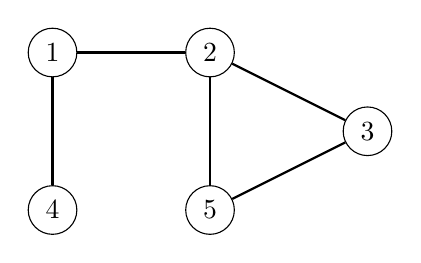
\begin{tikzpicture}
\node[draw, circle] (1) at (1,5) {$1$};
\node[draw, circle] (2) at (3,5) {$2$};
\node[draw, circle] (3) at (5,4) {$3$};
\node[draw, circle] (4) at (1,3) {$4$};
\node[draw, circle] (5) at (3,3) {$5$};

\path[draw,thick,-] (1) -- (2);
\path[draw,thick,-] (2) -- (3);
\path[draw,thick,-] (1) -- (4);
\path[draw,thick,-] (3) -- (5);
\path[draw,thick,-] (2) -- (5);
\end{tikzpicture}
\end{center}
می‌توان جستجو را از هر گره‌ای در گراف آغاز کرد؛
اکنون جستجو را از گره ۱ آغاز می‌کنیم.

جستجو ابتدا به گره ۲ پیش می‌رود:
\begin{center}
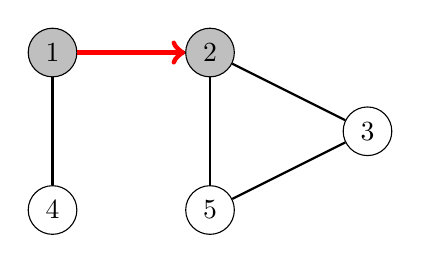
\begin{tikzpicture}
\node[draw, circle,fill=lightgray] (1) at (1,5) {$1$};
\node[draw, circle,fill=lightgray] (2) at (3,5) {$2$};
\node[draw, circle] (3) at (5,4) {$3$};
\node[draw, circle] (4) at (1,3) {$4$};
\node[draw, circle] (5) at (3,3) {$5$};

\path[draw,thick,-] (1) -- (2);
\path[draw,thick,-] (2) -- (3);
\path[draw,thick,-] (1) -- (4);
\path[draw,thick,-] (3) -- (5);
\path[draw,thick,-] (2) -- (5);

\path[draw=red,thick,->,line width=2pt] (1) -- (2);
\end{tikzpicture}
\end{center}
پس از آن، گره‌های ۳ و ۵ ملاقات خواهند شد:
\begin{center}
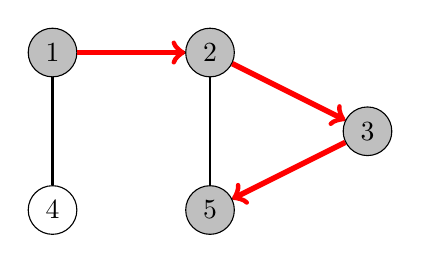
\begin{tikzpicture}
\node[draw, circle,fill=lightgray] (1) at (1,5) {$1$};
\node[draw, circle,fill=lightgray] (2) at (3,5) {$2$};
\node[draw, circle,fill=lightgray] (3) at (5,4) {$3$};
\node[draw, circle] (4) at (1,3) {$4$};
\node[draw, circle,fill=lightgray] (5) at (3,3) {$5$};

\path[draw,thick,-] (1) -- (2);
\path[draw,thick,-] (2) -- (3);
\path[draw,thick,-] (1) -- (4);
\path[draw,thick,-] (3) -- (5);
\path[draw,thick,-] (2) -- (5);

\path[draw=red,thick,->,line width=2pt] (1) -- (2);
\path[draw=red,thick,->,line width=2pt] (2) -- (3);
\path[draw=red,thick,->,line width=2pt] (3) -- (5);
\end{tikzpicture}
\end{center}
همسایه‌های رأس ۵ گره‌های ۲ و ۳ هستند،
ولی جستجو هر دو را قبلاً پیمایش کرده است.
زمان بازگشت به گره‌های قبلی فرارسیده است.
همسایه‌های گره‌های ۳ و ۲ نیز
پیمایش شده‌اند، پس مسیر بعدی
از گره ۱ به گره ۴ است:
\begin{center}
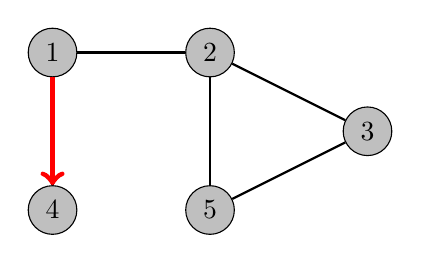
\begin{tikzpicture}
\node[draw, circle,fill=lightgray] (1) at (1,5) {$1$};
\node[draw, circle,fill=lightgray] (2) at (3,5) {$2$};
\node[draw, circle,fill=lightgray] (3) at (5,4) {$3$};
\node[draw, circle,fill=lightgray] (4) at (1,3) {$4$};
\node[draw, circle,fill=lightgray] (5) at (3,3) {$5$};

\path[draw,thick,-] (1) -- (2);
\path[draw,thick,-] (2) -- (3);
\path[draw,thick,-] (1) -- (4);
\path[draw,thick,-] (3) -- (5);
\path[draw,thick,-] (2) -- (5);

\path[draw=red,thick,->,line width=2pt] (1) -- (4);
\end{tikzpicture}
\end{center}
سپس جستجو پایان می‌پذیرد؛ همه گره‌ها
دیده شده‌اند.

پیچیدگی زمانی جستجوی اول‌عمق $O(n+m)$ است
که $n$ شمار گره‌ها و $m$ شمار
یال‌هاست،
زیرا الگوریتم هر گره و یال را یک بار بررسی می‌کند.

\subsubsection*{پیاده‌سازی}

جستجوی اول‌عمق به سادگی
با بازگشت پیاده‌سازی می‌شود.
تابع \texttt{dfs} زیر جستجوی اول‌عمق
را از گره داده‌شده آغاز می‌کند.
فرض تابع: گراف
به فرم لیست مجاورت در آرایه نگهداری شده است:
\begin{lstlisting}
vector<int> adj[N];
\end{lstlisting}
و آرایه‌ای دارد:
\begin{lstlisting}
bool visited[N];
\end{lstlisting}
که گره‌های پیمایش‌شده را ذخیره می‌کند.
ابتدا همه مقادیر آرایه \texttt{false} هستند؛
با رسیدن جستجو به گره $s$،
مقدار \texttt{visited}[$s$] برابر \texttt{true} می‌شود.
پیاده‌سازی تابع:
\begin{lstlisting}
void dfs(int s) {
    if (visited[s]) return;
    visited[s] = true;
    // process node s
    for (auto u: adj[s]) {
        dfs(u);
    }
}
\end{lstlisting}

\section{جستجوی اول‌سطح}

\index{breadth-first search}

\key{جستجوی اول‌سطح} (BFS) گره‌ها را
به ترتیب افزایش فاصله از گره آغازین
بررسی می‌کند.
از این رو، فاصله از گره آغازین
به سایر گره‌ها با جستجوی اول‌سطح
به دست می‌آید.
البته پیاده‌سازی جستجوی اول‌سطح
سخت‌تر از جستجوی اول‌عمق است.

جستجوی اول‌سطح گره‌ها را
سطح به سطح پیمایش می‌کند.
نخست گره‌های با فاصله ۱
از گره مبدأ،
سپس گره‌های با فاصله ۲ و همین ترتیب ادامه می‌یابد.
روند تا مشاهده تمام گره‌ها
ادامه دارد.

\subsubsection*{مثال}

بررسی عملکرد جستجوی اول‌سطح
روی گراف زیر:

\begin{center}
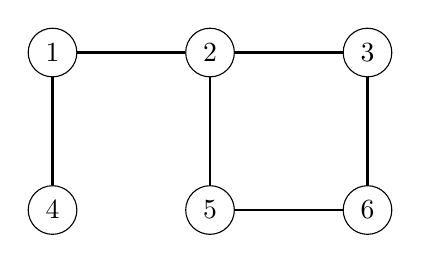
\begin{tikzpicture}
\node[draw, circle] (1) at (1,5) {$1$};
\node[draw, circle] (2) at (3,5) {$2$};
\node[draw, circle] (3) at (5,5) {$3$};
\node[draw, circle] (4) at (1,3) {$4$};
\node[draw, circle] (5) at (3,3) {$5$};
\node[draw, circle] (6) at (5,3) {$6$};

\path[draw,thick,-] (1) -- (2);
\path[draw,thick,-] (2) -- (3);
\path[draw,thick,-] (1) -- (4);
\path[draw,thick,-] (3) -- (6);
\path[draw,thick,-] (2) -- (5);
\path[draw,thick,-] (5) -- (6);
\end{tikzpicture}
\end{center}
فرض کنید جستجو از گره ۱ آغاز می‌شود.
ابتدا همه گره‌هایی را که می‌توان با یک یال از گره ۱ به آن‌ها رسید، پردازش می‌کنیم:
\begin{center}
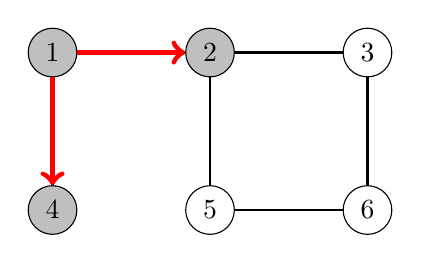
\begin{tikzpicture}
\node[draw, circle,fill=lightgray] (1) at (1,5) {$1$};
\node[draw, circle,fill=lightgray] (2) at (3,5) {$2$};
\node[draw, circle] (3) at (5,5) {$3$};
\node[draw, circle,fill=lightgray] (4) at (1,3) {$4$};
\node[draw, circle] (5) at (3,3) {$5$};
\node[draw, circle] (6) at (5,3) {$6$};

\path[draw,thick,-] (1) -- (2);
\path[draw,thick,-] (2) -- (3);
\path[draw,thick,-] (1) -- (4);
\path[draw,thick,-] (3) -- (6);
\path[draw,thick,-] (2) -- (5);
\path[draw,thick,-] (5) -- (6);

\path[draw,thick,-] (1) -- (2);
\path[draw,thick,-] (2) -- (3);
\path[draw,thick,-] (1) -- (4);
\path[draw,thick,-] (2) -- (5);

\path[draw=red,thick,->,line width=2pt] (1) -- (2);
\path[draw=red,thick,->,line width=2pt] (1) -- (4);
\end{tikzpicture}
\end{center}
پس از آن، به گره‌های ۳ و ۵ می‌رویم:
\begin{center}
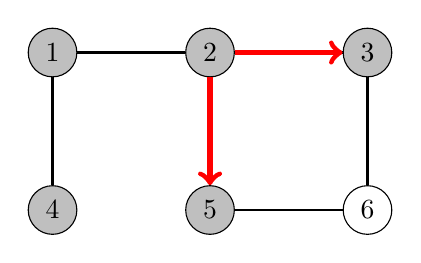
\begin{tikzpicture}
\node[draw, circle,fill=lightgray] (1) at (1,5) {$1$};
\node[draw, circle,fill=lightgray] (2) at (3,5) {$2$};
\node[draw, circle,fill=lightgray] (3) at (5,5) {$3$};
\node[draw, circle,fill=lightgray] (4) at (1,3) {$4$};
\node[draw, circle,fill=lightgray] (5) at (3,3) {$5$};
\node[draw, circle] (6) at (5,3) {$6$};

\path[draw,thick,-] (1) -- (2);
\path[draw,thick,-] (2) -- (3);
\path[draw,thick,-] (1) -- (4);
\path[draw,thick,-] (3) -- (6);
\path[draw,thick,-] (2) -- (5);
\path[draw,thick,-] (5) -- (6);

\path[draw,thick,-] (1) -- (2);
\path[draw,thick,-] (2) -- (3);
\path[draw,thick,-] (1) -- (4);
\path[draw,thick,-] (2) -- (5);

\path[draw=red,thick,->,line width=2pt] (2) -- (3);
\path[draw=red,thick,->,line width=2pt] (2) -- (5);
\end{tikzpicture}
\end{center}
در نهایت، گره ۶ را پیمایش می‌کنیم:
\begin{center}
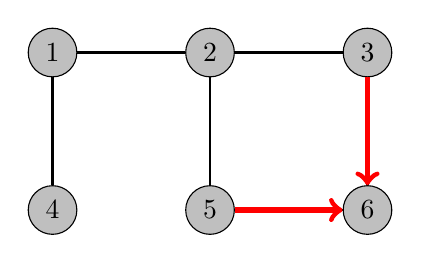
\begin{tikzpicture}
\node[draw, circle,fill=lightgray] (1) at (1,5) {$1$};
\node[draw, circle,fill=lightgray] (2) at (3,5) {$2$};
\node[draw, circle,fill=lightgray] (3) at (5,5) {$3$};
\node[draw, circle,fill=lightgray] (4) at (1,3) {$4$};
\node[draw, circle,fill=lightgray] (5) at (3,3) {$5$};
\node[draw, circle,fill=lightgray] (6) at (5,3) {$6$};

\path[draw,thick,-] (1) -- (2);
\path[draw,thick,-] (2) -- (3);
\path[draw,thick,-] (1) -- (4);
\path[draw,thick,-] (3) -- (6);
\path[draw,thick,-] (2) -- (5);
\path[draw,thick,-] (5) -- (6);

\path[draw,thick,-] (1) -- (2);
\path[draw,thick,-] (2) -- (3);
\path[draw,thick,-] (1) -- (4);
\path[draw,thick,-] (2) -- (5);

\path[draw=red,thick,->,line width=2pt] (3) -- (6);
\path[draw=red,thick,->,line width=2pt] (5) -- (6);
\end{tikzpicture}
\end{center}
اکنون فاصله‌ها را از گره آغازین تا همه گره‌های گراف محاسبه کرده‌ایم.
فاصله‌ها به شرح زیر است:

\begin{tabular}{ll}
\\
گره & فاصله \\
\hline
1 & 0 \\
2 & 1 \\
3 & 2 \\
4 & 1 \\
5 & 2 \\
6 & 3 \\
\\
\end{tabular}

مانند جستجوی اول‌سطح، پیچیدگی زمانی جستجوی اول‌سطح
برابر با $O(n+m)$ است، که در آن $n$ شمار گره‌ها
و $m$ شمار یال‌ها است.

\subsubsection*{پیاده‌سازی}

پیاده‌سازی جستجوی اول‌سطح از جستجوی اول‌عمق دشوارتر است،
زیرا الگوریتم، گره‌ها را در بخش‌های گوناگون گراف پیمایش می‌کند.
یک پیاده‌سازی متداول بر پایه یک صف شامل گره‌ها انجام می‌شود.
در هر گام، گره بعدی در صف پردازش می‌شود.

کد زیر فرض می‌کند گراف به صورت لیست‌های مجاورت ذخیره شده است
و داده‌ساختارهای زیر را نگهداری می‌کند:
\begin{lstlisting}
queue<int> q;
bool visited[N];
int distance[N];
\end{lstlisting}

صف \texttt{q} شامل گره‌هایی است که باید به ترتیب صعودی فاصله‌شان
پردازش شوند. گره‌های تازه همواره به انتهای صف افزوده می‌شوند
و گره ابتدای صف، گره بعدی برای پردازش است.
آرایه \texttt{visited} نشان می‌دهد کدام گره‌ها پیش‌تر توسط جستجو دیده شده‌اند،
و آرایه \texttt{distance} شامل فاصله‌ها از گره آغازین به تمام گره‌های گراف خواهد بود.

جستجو را می‌توان با شروع از گره $x$ به صورت زیر پیاده‌سازی کرد:
\begin{lstlisting}
visited[x] = true;
distance[x] = 0;
q.push(x);
while (!q.empty()) {
    int s = q.front(); q.pop();
    // process node s
    for (auto u : adj[s]) {
        if (visited[u]) continue;
        visited[u] = true;
        distance[u] = distance[s]+1;
        q.push(u);
    }
}
\end{lstlisting}

\section{کاربردها}

با استفاده از الگوریتم‌های پیمایش گراف،
می‌توان ویژگی‌های متعددی از گراف‌ها را بررسی کرد.
معمولاً هر دو الگوریتم جستجوی اول‌عمق و جستجوی اول‌سطح
قابل استفاده هستند، اما در عمل، جستجوی اول‌عمق
گزینه بهتری است زیرا پیاده‌سازی آن ساده‌تر است.
در کاربردهای زیر فرض می‌کنیم گراف بدون جهت است.

\subsubsection{بررسی همبندی}

\index{گراف همبند}

یک گراف همبند است اگر مسیری میان هر دو گره از گراف وجود داشته باشد.
بنابراین، می‌توان همبند بودن گراف را با شروع از یک گره دلخواه
و بررسی دسترسی‌پذیری به همه گره‌های دیگر ارزیابی کرد.

برای نمونه، در گراف
\begin{center}
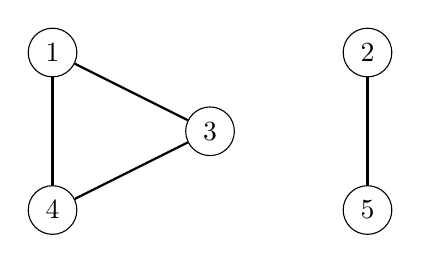
\begin{tikzpicture}
\node[draw, circle] (2) at (7,5) {$2$};
\node[draw, circle] (1) at (3,5) {$1$};
\node[draw, circle] (3) at (5,4) {$3$};
\node[draw, circle] (5) at (7,3) {$5$};
\node[draw, circle] (4) at (3,3) {$4$};

\path[draw,thick,-] (1) -- (3);
\path[draw,thick,-] (1) -- (4);
\path[draw,thick,-] (3) -- (4);
\path[draw,thick,-] (2) -- (5);
\end{tikzpicture}
\end{center}
یک جستجوی اول‌سطح‌عمق از گره $1$ گره‌های
زیر را پیمایش می‌کند:
\begin{center}
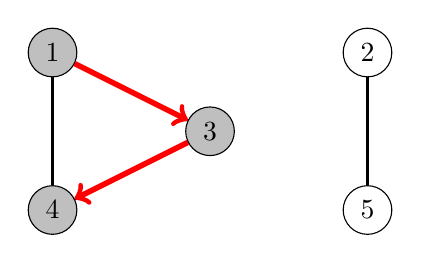
\begin{tikzpicture}
\node[draw, circle] (2) at (7,5) {$2$};
\node[draw, circle,fill=lightgray] (1) at (3,5) {$1$};
\node[draw, circle,fill=lightgray] (3) at (5,4) {$3$};
\node[draw, circle] (5) at (7,3) {$5$};
\node[draw, circle,fill=lightgray] (4) at (3,3) {$4$};

\path[draw,thick,-] (1) -- (3);
\path[draw,thick,-] (1) -- (4);
\path[draw,thick,-] (3) -- (4);
\path[draw,thick,-] (2) -- (5);

\path[draw=red,thick,->,line width=2pt] (1) -- (3);
\path[draw=red,thick,->,line width=2pt] (3) -- (4);

\end{tikzpicture}
\end{center}

از آنجا که جستجو همه گره‌ها را پیمایش نکرد،
می‌توان نتیجه گرفت که گراف همبند نیست.
به روش مشابه، می‌توان تمام مؤلفه‌های همبندی
یک گراف را نیز با پیمایش روی گره‌ها پیدا کرد؛ به این صورت که
اگر گره فعلی هنوز به هیچ مؤلفه‌ای تعلق ندارد،
همواره یک جستجوی اول‌سطح‌عمق جدید آغاز شود.

\subsubsection{یافتن دورها}

\index{دور}

یک گراف شامل دور است اگر هنگام پیمایش گراف،
گره‌ای پیدا کنیم که همسایه آن (غیر از
گره قبلی در مسیر فعلی) قبلاً پیمایش
شده باشد.
برای مثال، گراف
\begin{center}
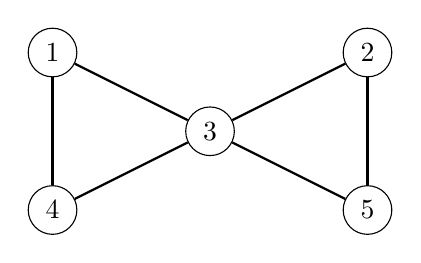
\begin{tikzpicture}
\node[draw, circle] (2) at (7,5) {$2$};
\node[draw, circle] (1) at (3,5) {$1$};
\node[draw, circle] (3) at (5,4) {$3$};
\node[draw, circle] (5) at (7,3) {$5$};
\node[draw, circle] (4) at (3,3) {$4$};

\path[draw,thick,-] (1) -- (3);
\path[draw,thick,-] (1) -- (4);
\path[draw,thick,-] (3) -- (4);
\path[draw,thick,-] (2) -- (5);
\path[draw,thick,-] (2) -- (3);
\path[draw,thick,-] (3) -- (5);
\end{tikzpicture}
\end{center}
دارای دو دور است و می‌توان یکی
از آنها را به صورت زیر پیدا کرد:
\begin{center}
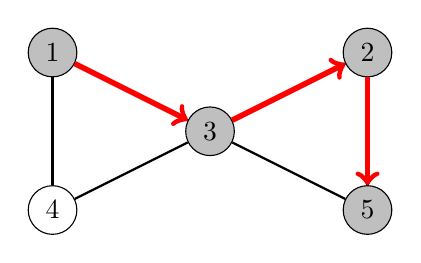
\begin{tikzpicture}
\node[draw, circle,fill=lightgray] (2) at (7,5) {$2$};
\node[draw, circle,fill=lightgray] (1) at (3,5) {$1$};
\node[draw, circle,fill=lightgray] (3) at (5,4) {$3$};
\node[draw, circle,fill=lightgray] (5) at (7,3) {$5$};
\node[draw, circle] (4) at (3,3) {$4$};

\path[draw,thick,-] (1) -- (3);
\path[draw,thick,-] (1) -- (4);
\path[draw,thick,-] (3) -- (4);
\path[draw,thick,-] (2) -- (5);
\path[draw,thick,-] (2) -- (3);
\path[draw,thick,-] (3) -- (5);

\path[draw=red,thick,->,line width=2pt] (1) -- (3);
\path[draw=red,thick,->,line width=2pt] (3) -- (2);
\path[draw=red,thick,->,line width=2pt] (2) -- (5);

\end{tikzpicture}
\end{center}
پس از حرکت از گره 2 به گره 5 متوجه می‌شویم که
همسایه 3 از گره 5 قبلاً پیمایش شده است.
بنابراین، گراف شامل دوری است که از گره 3 می‌گذرد،
برای مثال، $3 \rightarrow 2 \rightarrow 5 \rightarrow 3$.

روش دیگر برای تشخیص وجود دور در گراف،
محاسبه ساده تعداد رأس‌ها و یال‌ها در هر مؤلفه است.
اگر مؤلفه‌ای شامل $c$ رأس و فاقد دور باشد،
دقیقاً شامل $c-1$ یال است
(بنابراین باید یک درخت باشد).
اگر $c$ یا تعداد بیشتری یال وجود داشته باشد،
آن مؤلفه قطعاً شامل دور است.

\subsubsection{بررسی دوبخشی بودن}

\index{گراف دوبخشی}

یک گراف دوبخشی است اگر بتوان رأس‌های آن را با دو رنگ
به‌گونه‌ای رنگ‌آمیزی کرد که هیچ دو رأس مجاوری
هم‌رنگ نباشند.
بررسی دوبخشی بودن یک گراف با الگوریتم‌های پیمایش گراف
بسیار آسان است.

ایده کار رنگ کردن رأس شروع با رنگ آبی،
تمام همسایه‌های آن با رنگ قرمز، همسایه‌های آن‌ها با رنگ آبی، و به همین ترتیب است.
اگر در نقطه‌ای از جستجو مشخص شود که
دو رأس مجاور هم‌رنگ هستند،
گراف دوبخشی نیست.
در غیر این صورت، گراف دوبخشی است و یک رنگ‌آمیزی
یافت شده است.

برای مثال، گراف
\begin{center}
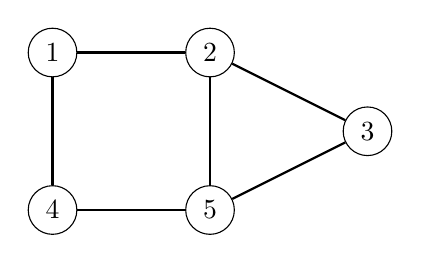
\begin{tikzpicture}
\node[draw, circle] (2) at (5,5) {$2$};
\node[draw, circle] (1) at (3,5) {$1$};
\node[draw, circle] (3) at (7,4) {$3$};
\node[draw, circle] (5) at (5,3) {$5$};
\node[draw, circle] (4) at (3,3) {$4$};

\path[draw,thick,-] (1) -- (2);
\path[draw,thick,-] (2) -- (5);
\path[draw,thick,-] (5) -- (4);
\path[draw,thick,-] (4) -- (1);
\path[draw,thick,-] (2) -- (3);
\path[draw,thick,-] (5) -- (3);
\end{tikzpicture}
\end{center}
دوبخشی نیست، زیرا جستجو از رأس ۱
به این صورت پیش می‌رود:
\begin{center}
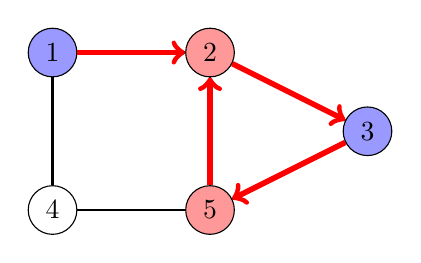
\begin{tikzpicture}
\node[draw, circle,fill=red!40] (2) at (5,5) {$2$};
\node[draw, circle,fill=blue!40] (1) at (3,5) {$1$};
\node[draw, circle,fill=blue!40] (3) at (7,4) {$3$};
\node[draw, circle,fill=red!40] (5) at (5,3) {$5$};
\node[draw, circle] (4) at (3,3) {$4$};

\path[draw,thick,-] (1) -- (2);
\path[draw,thick,-] (2) -- (5);
\path[draw,thick,-] (5) -- (4);
\path[draw,thick,-] (4) -- (1);
\path[draw,thick,-] (2) -- (3);
\path[draw,thick,-] (5) -- (3);

\path[draw=red,thick,->,line width=2pt] (1) -- (2);
\path[draw=red,thick,->,line width=2pt] (2) -- (3);
\path[draw=red,thick,->,line width=2pt] (3) -- (5);
\path[draw=red,thick,->,line width=2pt] (5) -- (2);
\end{tikzpicture}
\end{center}
مشاهده می‌شود که رنگ هر دو رأس ۲ و ۵
قرمز است، در حالی که این دو در گراف مجاور یکدیگرند.
بنابراین، گراف دوبخشی نیست.

این الگوریتم همواره کار می‌کند؛ زیرا با داشتن تنها دو رنگ،
رنگ رأس شروع در یک مؤلفه،
رنگ تمام رأس‌های دیگر آن مؤلفه را تعیین می‌کند.
قرمز یا آبی بودن رأس شروع
هیچ تفاوتی ایجاد نمی‌کند.

در حالت کلی،
تشخیص امکان رنگ‌آمیزی رأس‌های گراف با $k$ رنگ
به‌طوری که هیچ دو رأس مجاوری هم‌رنگ نباشند، دشوار است.
حتی برای $k=3$ نیز الگوریتم کارآمدی شناخته نشده
و مسئله NP-hard است.